\section{Inicializácia algoritmov}

Na inicializáciu Metropolis--Hastings metód (Hit--and--Run generátora a aj Gibbsovho generátora) je potrebný počiatočný bod vnútri polyédra a veľkosť burn--in periódy (iterácii algoritmu bez vracania vygenerovaných bodov ako výsledkov). Ako počiatočný bod sme zvolili bod $c$ určený pri generovaní polyédra, ktorý je vygenerovaný na prieniku polyédra a jednotkovej hyperkocky rovnomerne náhodne. Vzhľadom k tomu, že generujeme veľké množstvo bodov v polyédri, je burn--in perióda nepotrebná. Symbolicky bola zvolená hodnota $100$.

Na inicializáciu zamietacej metódy pomocou MVEE elipsoidu je potrebné vypočítať MVEE elipsoid. Pri inicializácii REX algoritmu je potrebné zvoliť počiatočný nosič tak, aby bola informačná matica $M$ regulárna. V rámci práce bol nosič počiatočného návrhu zvolený ako $n+1$ náhodných vrcholov. Vzhľadom na náhodnosť polyédra, dané vrcholy budú s pravdepodobnosťou $1$ určovať regulárnu maticu $M$.

\section{Porovnanie rýchlostí generovania}

V rámci testovania boli metódy porovnávané na rozmeroch $d=1, \dots, 9$, v každom rozmere bolo vygenerovaných $100$ náhodných polyédrov. Na každom z daných polyédrov boli spustené všetky metódy, každá z nich vygenerovala $10^5$ bodov vnútri polyédru. Ako výstup testovania boli pre každú metódu zobrazené priemerné rýchlosti generovaní bodov v jednotlivých rozmeroch.\\

\begin{figure}[H]
  \centering
  \begin{subfigure}[b]{\linewidth}
    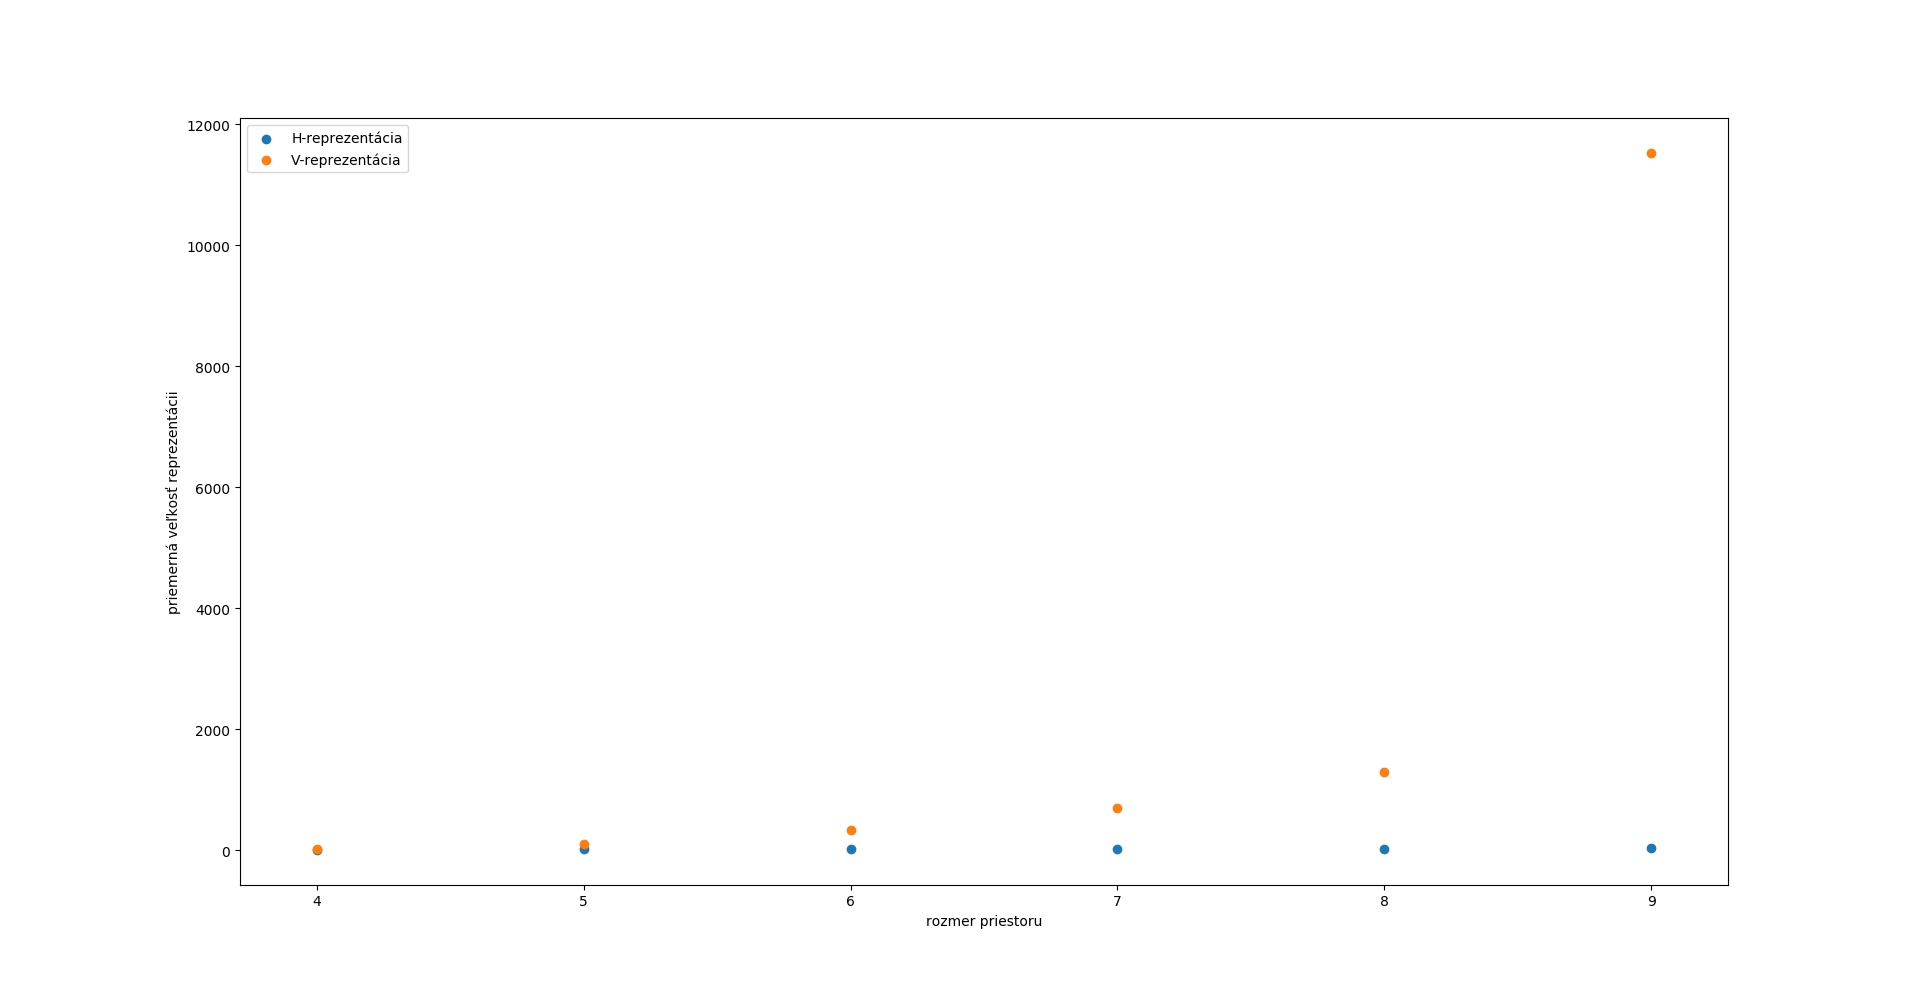
\includegraphics[width=0.9\linewidth]{images/velkost_rep.png}
    \caption{Priemerná veľkosť reprezentácií polyédrov vzhľadom na počet rozmerov priestoru}
	\label{fig:velkost_rep}
  \end{subfigure}
  \begin{subfigure}[b]{\linewidth}
    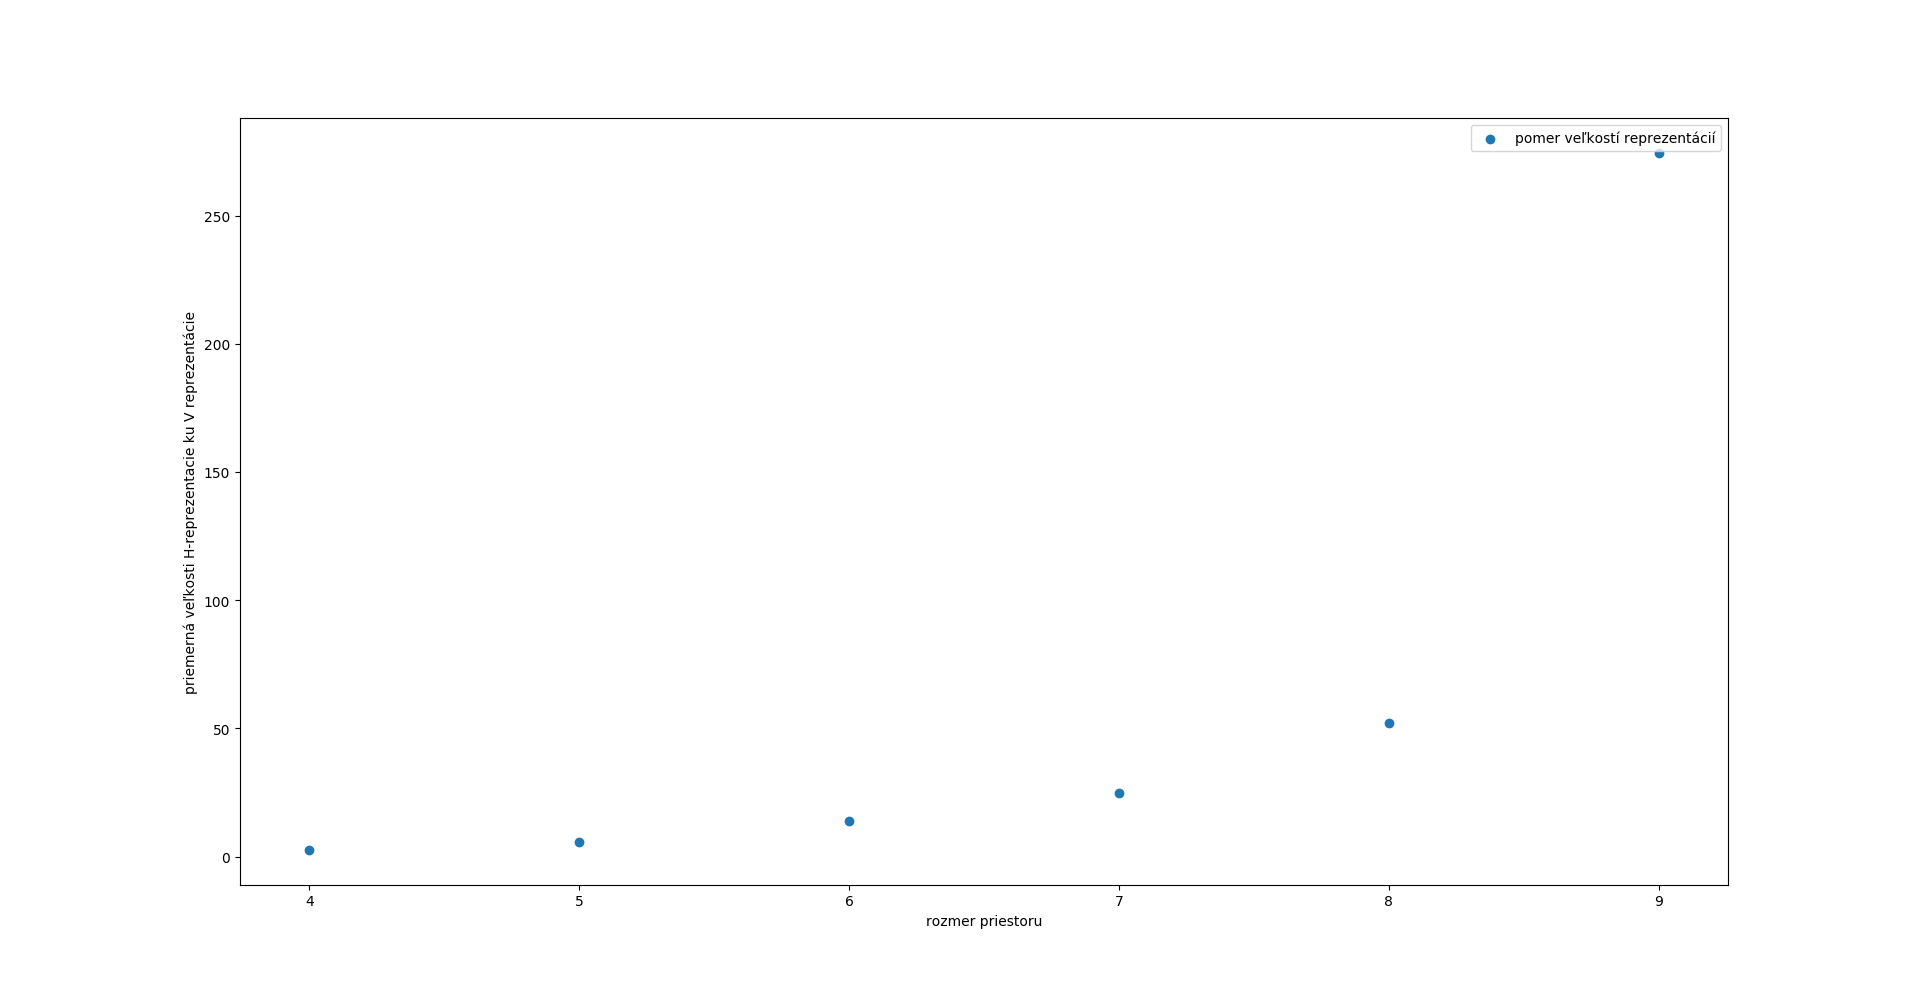
\includegraphics[width=0.9\linewidth]{images/pomer_rep.png}
    \caption{Pomer veľkostí reprezentácii polyédrov vzhľadom na počet rozmerov priestoru}
	\label{fig:pomer_rep}
  \end{subfigure}
  \caption{Reprezentácie polyédra}
\end{figure}

Pozrime sa najprv na nami vygenerované ``náhodné'' polyédre. Pozrime sa na priemerné veľkosti reprezentácii nami ``náhodne'' vygenenerovaných polyédrov (viď \ref{fig:velkost_rep}). Očividne očakávaný rozdiel veľkostí reprezentácii so zvyšujúcim sa rozmerom priestoru rastie. Taktiež pomer $\frac{\text{veľkosť V--reprezentácie}}{\text{veľkosť H--reprezentácie}}$ so zvyšujúcim sa rozmerom priestoru rastie (viď \ref{fig:pomer_rep}).

Zväčšenie V--reprezentácie zjavne spomalí nájdenie MVEE (REX algoritmu). Okrem toho nám veľká V--reprezentácia pri porovnávaní algoritmov nerobí žiaden iný problém. Pri vypočítanom MVEE je už beh MVEE metódy nezávislý od veľkosti V--reprezentácie (je závislý jedine od matíc $A$, $C$ a vektorov $b$ a $\mathbf{\overline z}$).\\

\begin{figure} [H]
	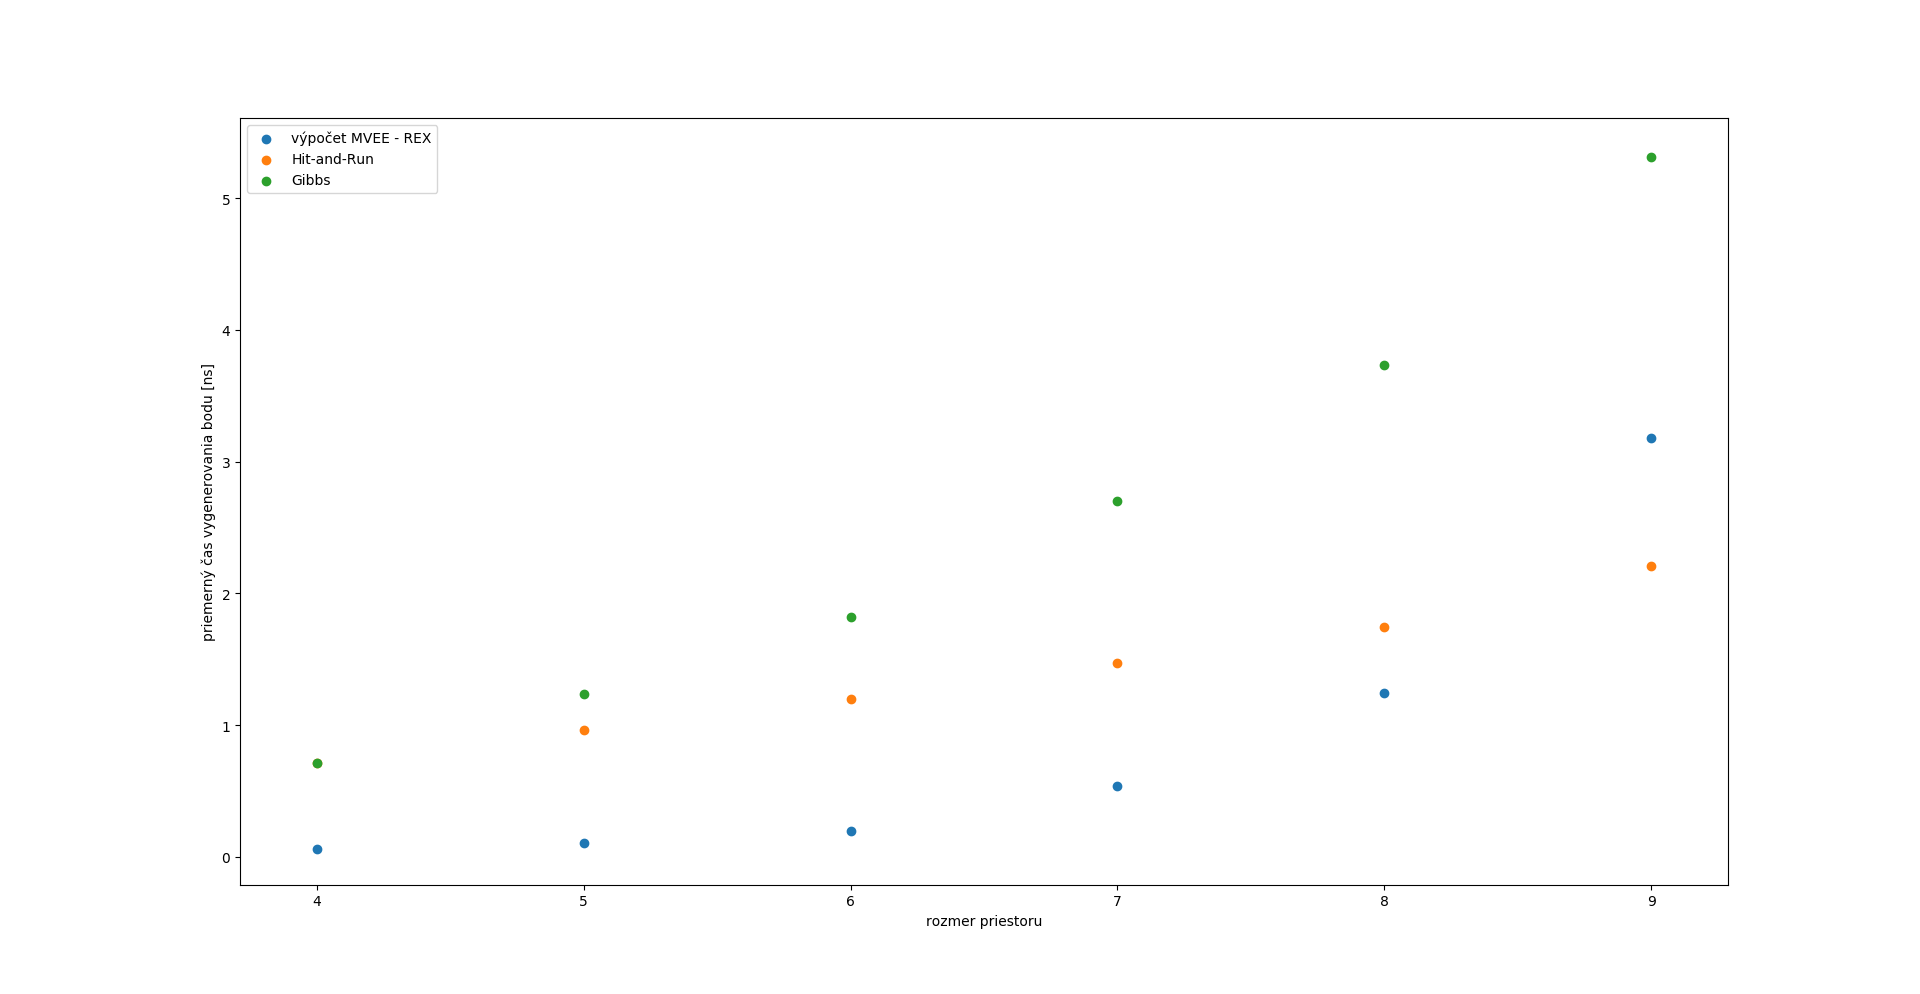
\includegraphics[width=\linewidth]{images/mh_rex.png}
	\caption{Porovnanie priemerného vygenerovania bodu Metropolis--Hasting metódou s výpočtom MVEE pomocou REX algoritmu vzhľadom na počet rozmerov priestoru}
	\label{fig:mh_rex}
\end{figure}

Keď sa pozrieme na priemerný čas výpočtu REX algoritmu (viď \ref{fig:mh_rex}), je porovnateľný s očakávaným časom trvania vygenerovania jedného bodu pomocou Metropolis--Hastings metód. Nakoľko pri danom polyédri je REX použitý práve raz, očakávaný čas trvania REXu je pri porovnávaní metód zanedbateľný.\\

\begin{figure} [H]
  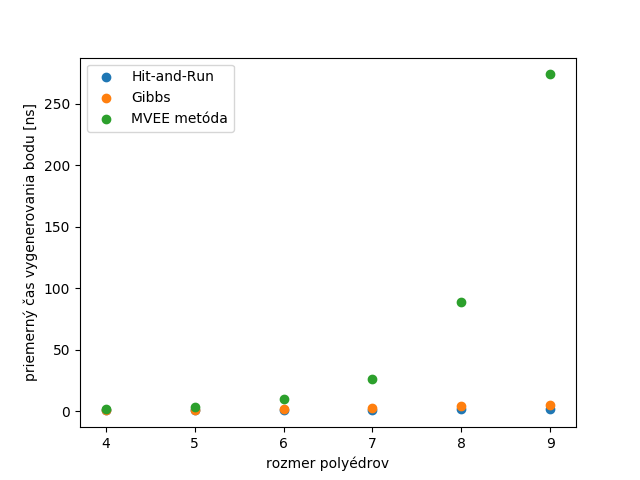
\includegraphics[width=\linewidth]{images/vsetky.png}
  \caption{Priemerný čas trvania všetkých metód}
  \label{fig:vsetky}
\end{figure}

Metóda MVEE pri vyššom počte rozmerov generuje body výrazne pomalšie ako Metropolis--Hastings metódy (viď \ref{fig:vsetky}).
To musí byť spôsobené zväčšením pomeru objemov $\frac{\lambda(T_{MVEE})}{\lambda(S)}$. Preto náš horný odhad $d^d$ očakávaného počtu generovaní (kde $d$ je počet rozmerov priestoru) podľa Johnovho elipsoidu nemusí byť tak voľný, ako sa na prvý pohľad zdá.\\

\begin{figure} [H]
	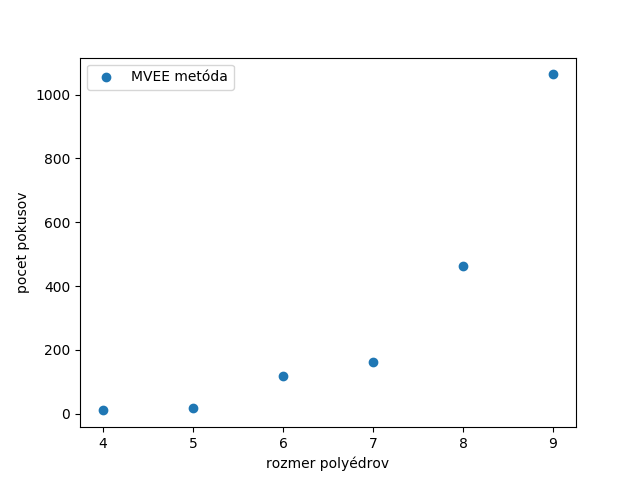
\includegraphics[width=\linewidth]{images/mvee_pokusy.png}
	\caption{Priemerný počet pokusov na nájdenie bodu v polyédri pomocou MVEE vzhľadom na počet rozmerov priestoru}
	\label{fig:mvee_pokusy}
\end{figure}

Odhadnime, ako dobre MVEE obaľuje polyéder $S$ v $d$--rozmernom priestore. Ozačme si priemerný počet pokusov na vygenerovanie bodu v polyédri rozmeru $d$ ako $E(S)$. Hodnotu $E(S)$ máme vypočítanú z MVEE metódy. Kedže platí $E(S)=\frac{\lambda(T_{MVEE})}{\lambda(S)}$, možno odhadnúť pomer $\frac{\lambda(T_{MVEE})}{\lambda(S)}$ pomocou $E(S)$. Z grafu \ref{fig:mvee_pokusy} vidno, že počet pokusov na vygenerovanie bodu v polyédri pomocou MVEE metódy s rastúcim počtom rozmerov rastie, preto ``tesnosť'' obalu MVEE polyédra $S$ s rastúcim počtom rozmerov klesá.

Tiež si všimnime, že pomocou $E(S)$ možno odhadnúť aj objem $\lambda(S)$. Platí $$\lambda(S)=\frac{\lambda(T_{MVEE})}{E(S)}=\frac{\lambda(V_d) \cdot \text{det}(C)}{E(S)},$$ kde $V_d$ je objem $d$--rozmernej jednotkovej gule a $C$ je matica taká, že MVEE prislúchajúci k $S$ je $=E(\mathbf{\overline H, \overline z})=E((CC^T)^{-1}, \mathbf{ \overline z})$.

\begin{figure} [H]
  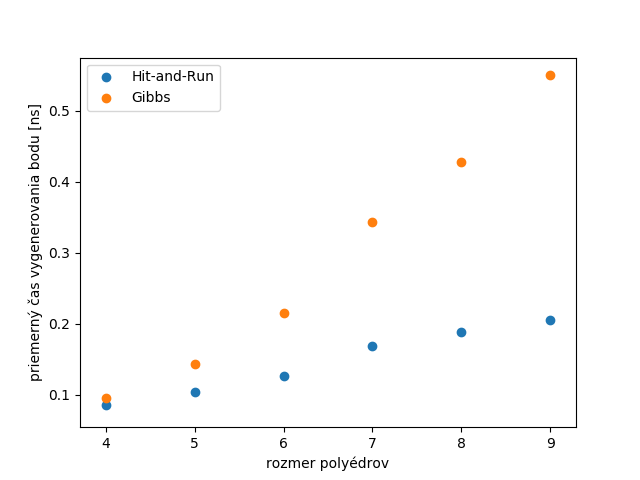
\includegraphics[width=\linewidth]{images/mh.png}
  \caption{Priemerný čas trvania generovania bodov Metropolis--Hastings metód}
  \label{fig:mh}
\end{figure}

Porovnanie Metropolis--Hastings metód dopadlo podľa očakávaní. Čas potrebný na vygenerovanie bodu pomocou Gibbsovho generátor rástol asymptoticky kvadraticky a čas potrebný na vygenerovanie bodu pomocou Hit--and--Run generátora rástol asymptoticky lineárne (viď \ref{fig:mh}).\\

\section{Výsledky porovnania}

Z daných porovnaní vyplýva, že najrýchlejší algoritmus na generovanie veľkého počtu bodov z rovnomerného rozdelenia vo veľarozmernom polyédri je generátor Hit--and--Run.

Zamietacia metóda pomocou MVEE je pri väčšom rozmere priestoru kvôli veľkému pomeru $\frac{\lambda(T_{MVEE})}{\lambda(S)}$ nepoužiteľná.\\

Je potrebné podotknúť, že síce Metropolis--Hasting metódy (špeciálne aj Hit--and--Run generátor) sú pri väčšom počte rozmerov značne rýchlejšie ako zamietacia metóda pomocou MVEE, no na druhú stranu, taktiež majú oproti MVEE metóde pri použití v praxi relevantnú nevýhodu. Totiž pri MVEE metóde sú vygenerované body priamo z rovnomerného rozdelenia na polyédri, no pri Metropolis--Hastings metódach rozdelenie postupnosti vygenerovaných bodov iba limitne konverguje k žiadanému rozdeleniu.

Preto MVEE metóda môže byť lepšou voľbou v určitých prípadoch (menší rozmer polyédra, menší požadovaný počet realizácií alebo nutnosť dodržať úplne presné rovnomerné rozdelenie). Taktiež, MVEE metóda je vhodná, ak je potrebné vypočítať intervaly spoľahlivosti pre objem daného polyédra. 